\chapter{提案手法}

\section{Web文書を用いたクエリゆう度モデルの拡張}
前章で述べたスムージングを用いながら,Web文書による情報量の拡張を図る.式(7.1)にWeb文書を併用したクエリゆう度モデルの式を示す.

\begin{flalign}
    & P(w_i|\theta_d; \alpha; \mu; \nu) = \nonumber \\ 
    & \frac{\alpha}{\alpha+\mu+\nu} P(w_i|\theta_d)
    &+ \frac{\mu}{\alpha+\mu+\nu} P(w_i|\theta_D)
    &+ \frac{\nu}{\alpha+\mu+\nu} P(w_i|\theta_W)  
    \label{eq_expanddirichlet}
\end{flalign}

ここで $P(w_i│θ_W)$はWeb文書集合 $W$ 内での語 $w_i$ の生起確率である.同様に $P(w_i│θ_D)$ は文書コレクション $D$ 内,$P(w_i│θ_d)$ は検索対象文書 $d$ 内の $w_i$ の生起確率である.また,$\alpha$, $\mu$, $\nu$はスムージングパラメータである.Web文書として,本研究では次節に倣い,各質問クエリから名詞情報を抽出して検索を行った結果を用いている. 

\subsection{Web 文書の取得}
Web文書の取得方法は,まず各クエリの単語に対してTF-IDF値を計算し,TF-IDF値のスコアの上位5単語を抽出する.そして,5単語から3単語を取り出す全て組み合わせおいて,Web検索を行い,各検索に対し10件のWeb文書を取得する.そのため,1クエリに対し,Web文書を100件取得した.最後に得られたWeb文書全てを,1つの巨大な文書とみなし,$P(w_i│θ_W)$ を計算し,式(7.1)で利用する.
ここでIDFの計算に文書コレクションを利用した.

\section{評価実験}
\subsection{実験条件}
提案手法の有用性を示すため,評価実験を行なった.Web文書をクエリ尤度モデルのスムージングに利用した式(8.1)を用いた場合(スムージングパラメータ: $\alpha$ = 0.5, $\mu$ = 0.3, $\nu$ = 0.2)とWeb文書を利用せず,スムージングに文書コレクションのみを利用した場合(スムージングパラメータ: $\alpha$ = 0.5, $\mu$ = 0.5, $\nu$ = 0.0)のMAP値を比較し,本手法の有用性を調べた.また,クエリの長さに応じたMAP値の変化も調査した.ここでクエリの長さは,クエリ内に存在する名詞の個数とする.クエリの長さに応じて4分割した際の各集合の条件を表7.1に纏める.

\begin{table}
    \centering
    \caption{クエリを分割したときに各集合}
    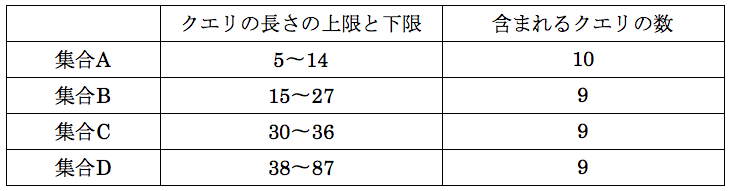
\includegraphics[width=7cm]{./image/query_set.png}
    \label{query_set}
\end{table}

\subsection{実験結果}
実験結果を図7.1に示す.

\begin{figure}
    \centering
    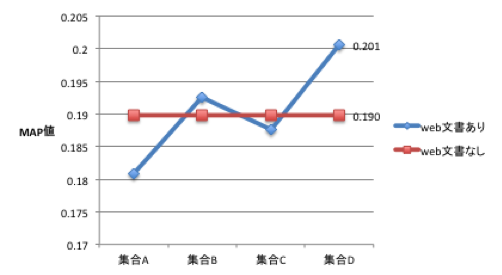
\includegraphics[width=7cm]{./image/web_result.png}
    \caption{Web文書を利用したときのMAP値}
    \label{web_result1}
\end{figure}

図7.1よりWeb文書を用いた本手法のMAP値の最大値は,Web文書を利用していない場合より高くなった.またクエリが長いほど本手法のMAP値は上昇した.これは,クエリが長いほど,文書コレクションだけではスムージングが対応できなくなり,Web文書によるスムージングが必要になるからだと考えられる.
